\chapter{Я долго это терпел, но хватит}




Я открою вам глаза. Повсюду при описании Греко-Персидских войн мы видим одно и тоже. Ужасные, грязные, немытые полчища персов лезут и лезут в няшную, прекрасную Грецию, огребают там заслуженных пиздюлей и откатываются назад, а потом вообще Сашка Македонский пришёл и покончил с этим нелепым Мордором во имя добра и справедливости. ЭТО НЕПРАВДА, ложь, пиздеж и ватная эллинская пропаганда. Политрук лжет, не читайте комиксы а читайте учебники, там про всё написано. Ну а я вам сейчас быстренько обрисую греко-персидские отношения. Выводы можете делать сами.


Конфликты начались не в Греции, куда откуда не возьмись прибежали персы. А в Малой Азии. Персидская империя была огромной, континентальной страной, разделенной на сатрапии. Так как бюрократии тогда ещё не было, то управлять столь здоровенными государственными образованиями в ручном режиме было нереально. И поэтому везде в огромной имперке был свой уклад. В том числе и на побережье Эгейского моря, где греки засирали всё своими колониями в тотал. Естественно, их тоже поглотила семья братских персидский народов, но им даже внутреннее устройство корежить не стали. Демократия значит демократия. Просто над вами, демократическими полисами, ещё будет стоять сатрап, представитель персидского царя, чтоб вы долю малую отстегивали наверх и вели себя хорошо. В общем, было более чем нормально. Но однажды, пока царь в другом конце государства с кем-то воевал, местные греки чёт не поделили с местным сатрапом. Вроде как планировали совместную операцию, но переругались, операцию сорвали и остались друг другом крайне недовольные. А войска-то собраны... ну и началось восстание, собственно говоря, которое быстро перекинулось на остальные, всегда любившие помайданить, города. Причём греки, пользуясь моментом, начали проводить перераспределение капиталов, резать персов и отжимать у них имущество, а ещё пригласили в свою страну интервентов-афинян, которые радостно вписались в движ и начали творить всякое гуро. В том числе сожгли какой-то важный для персов храм и всех там убили, что вообщет абсолютно неприемлемо.


Но потом вернулся царь персов, всех там перехерачил, и майданить греки Малой Азии прекратили. Однако остались ещё Афины, которые тоже следовало наказать. Для чего, тихой сапой, начинается подчинение Македонии, и персидское влияние переваливается через Босфор. Затем, собственно, происходит вообще феерическая херня. Персам было важно как-то обуздать эллинов, которые везде плавали и все грабили-убивали, что в прибрежной зоне находится. Для чего к ним отправляется посольство, которое не требует чего-то сверхординарного. Просто от афинян требуют принести извинения за прошлый беспредел, номинальное признать власть персидского царя и сказать "мы больше так не будем". Всё. Чем отвечают Афины? Они убивают послов (полный, тотальный беспредел, на который способна только демократия) и скидывают их в колодец. Да, спартанцы не при делах, это Афины. И только после этого не то чтобы миролюбивая, но не разменивающаяся на херню Персидская держава решает что надо отвечать жёстко, и прекращать этот балаган. Случается знаменитая битва при Марафоне, и Афины кое-как откидываются, громя экспедиционный корпус персов. На этом первая фаза войны заканчивается, греки решают что не надо дразнить Тигра, а у персов начинается усобица и им просто не до того.


Проходят годы, греки смелеют, и опять начинают вытворять на море всякую хуйню, чем опять вынуждают персов реагировать. Персы собирают огромную армию, и уже во главе с царём вторгаются в Элладу через Македонию. Армия реально большая, она прёт на Афины, и, при Фермопилах сносит жидкий заслон из спартанцев и примкнувших к ним других греков. Там задержка было в 2-3 дня, и это реально ничего не решало. После Фермопил персы идут дальше, подходят к пустым Афинам и сжигают их нахер, что, в общем-то, справедливо. А дальше случается НЕОЖИДАННЫЙ ПОВОРОТ. Афиняне эвакуировали город заранее и сохранили флот, и эти флотом они заманивают эскадру персов и при Саламине выносят её начисто. А после этого сухопутная армия персов, оставшись без снабжения, вынуждена отступать как Наполеон от Москвы.


И если вы думаете что это всё, то нет. После этого Афины, под предлогом защиты от персов, сгребают всех греков в единый союз, и требуют с них всех дань, где войсками а где деньгами, отчего быстро богатеют и начинают "годы морского разбоя" в Средиземном Море. Персы мучительно восстанавливают флот, а Афины, безнаказанно, выжигают побережье империи. Этот адок длился годами: сатрапии неповоротливы, а сухопутных армии медленные. А афиняне всё грабят и выжигают, что твои викинги. В общем, тяжёлое было время. Но потом Афины заигрались и залезли почти всем своим флотом в устье Нила. Где их и встретили, загнали в один из рукавов и осадили на острове. Египтяне, для которых Нил это святая река, осушают русло, настолько Афины всех заебали. И весь экспедиционный корпус вырезают. НАКОНЕЦ-ТО, ептеть. После чего на море наступает относительный паритет в силах, и разграбление империи прекращается. А потом цивилизованные персы смотрят как Афины в Греции всех тиранят, и без всякой войны, чисто за бабло, начинают шатать Афинский союз, и двигать в гегемоны Спарту. И когда спартанцы, на персидские деньги, вломили Афинам пизды, империя вздохнула спокойно. Теперь ебучие варвары с Эллады будут очень долго меряться у кого член больше, пока их всех Македония не зажует и Македонский не начнёт свои завоевания.

\begin{figure}[h!tb] 
	\centering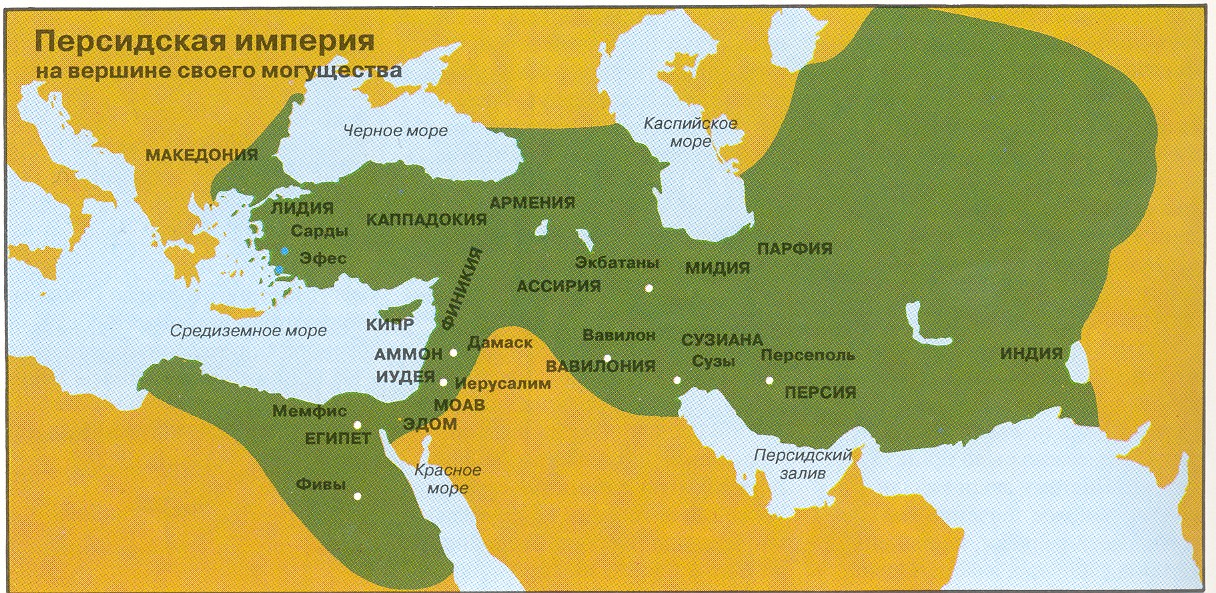
\includegraphics[scale=0.3]{FFFAtit/1576580368153797925.png}
	%	\label{fig:scipion} % Unique label used for referencing the figure in-text\end{document}
	%	%\addcontentsline{toc}{figure}{Figure \ref{fig:placeholder}} % Uncomment to add the figure to the table of contents%----------------------------------------------------------------------------------------
	%	\caption{На пикчах ниже всякие вариации на тему "сенаторы убивают Салата".}%	CHAPTER 2
\end{figure}

Но и тут Сашка, разбив ополчение с персидские сатрапий и переподчинив их себе, посмотрит на свой трофей (там одно убранство царского дворца это несколько годовых бюджетов всей Эллады), и немедленно начнёт женить своих полководцев на местных, всячески косить под персов и пытаться как-то встроить свой сраный эллинизм в великую персидскую цивилизацию. Да, эллины умели воевать, но культурно там пропасть в века, если не в тысячелетия. А когда Сашка помрёт, то ты увидим закономерную двадцатилетнюю свалку за власть между Диадохами. А затем на карте останутся абсолютно египетское царство Птолемеев, и абсолютно персидская как по форме так и по содержанию империя Селевкидов. Обе с лёгкими вкраплениями эллинизма. Вот так вот две великие восточные цивилизации за ничтожный по историческим меркам срок переварили захватчиков, кооптировали их в себя и отлично просуществовали пока их Рим всех не перебил. Но и тут не всё так просто, Египет вошёл в Республику последним и на условиях почти полной внутренней автономии. А Персия после гибели имперки Селевка вновь переродилась под крылом Парфии, и спокойно бодалась с Римом а потом и с Византией, пока их ислам всех не перехуярил. Да и там, если вы знаете чего такое шиизм и как он появился, то вы смекнете, что персидская история на этом нифига не закончилась.


А всё почему? Потомушта что устье Нила, что Междуречье, на момент столкновения с западными варварами, это тысячи лет непрерывной истории и культурной Традиции, это старейшие цивилизации на планете (Китай может поспорить, но он далековато будет), и нет ничего удивительного, что они обе что на греков, что на римлян смотрели как на говно и культурно ассимилировали, отучая вытирать жопу лопухом и приобщая к цивилизации. Удивительно то, что у нас это конфликт миров обычно переворачивают с ног а голову, и пирсингованный царь Ксеркс несёт ебучее варварство передовым европейским демократиям, лол.


